\section{General Results}
\label{GeneralResults}

%\subsection{General Aspects}
%\label{GeneralAspects}

% talk about the simulation in general terms, describing the parameters,
% features, how it matches observations, then lead into why we need
% a more quantitative language in describing the details of reionization

%In this paper, we analyze a simulation that serves as a test run for an upcoming large-scale %capability run.  As a result, the size of our computational domain is not representative of the %entire universe, but it is a good test case of the code's ability to simulate the desired physics in %a moderate amount of time on moderate computational resources.  We therefore take a physical %box size of 20 Mpc comoving,
%and choose initial conditions and cosmological parameters to match those of WMAP 7 data %\citep{JarosikEtAl2011}.  Although missing the higher power in the matter power spectrum, %which occurs on the scale of $\sim100$ Mpc comoving, we show that all the physics are correct %and behaving as expected.

%\begin{figure*}[ht]
%  \includegraphics[width=0.9\textwidth]{4_panel_HI_slice.png}
% \caption{H I density on slices through the 20 Mpc volume showing the growth, 
%percolation, and final overlap of HII regions. Panels show $z=9, 7.7,
%6.96, 6.3$. The box becomes fully ionized at z=6.13 as the last neutral islands
%are overrun by the I-fronts. Regions of extremely low HI density are shock-heated 
%bubbles due to supernova feedback.}
%  \label{HI_slices}
%\end{figure*}

\begin{figure*}[!tp]
    \begin{minipage}[h]{0.5\linewidth}
        \centering
        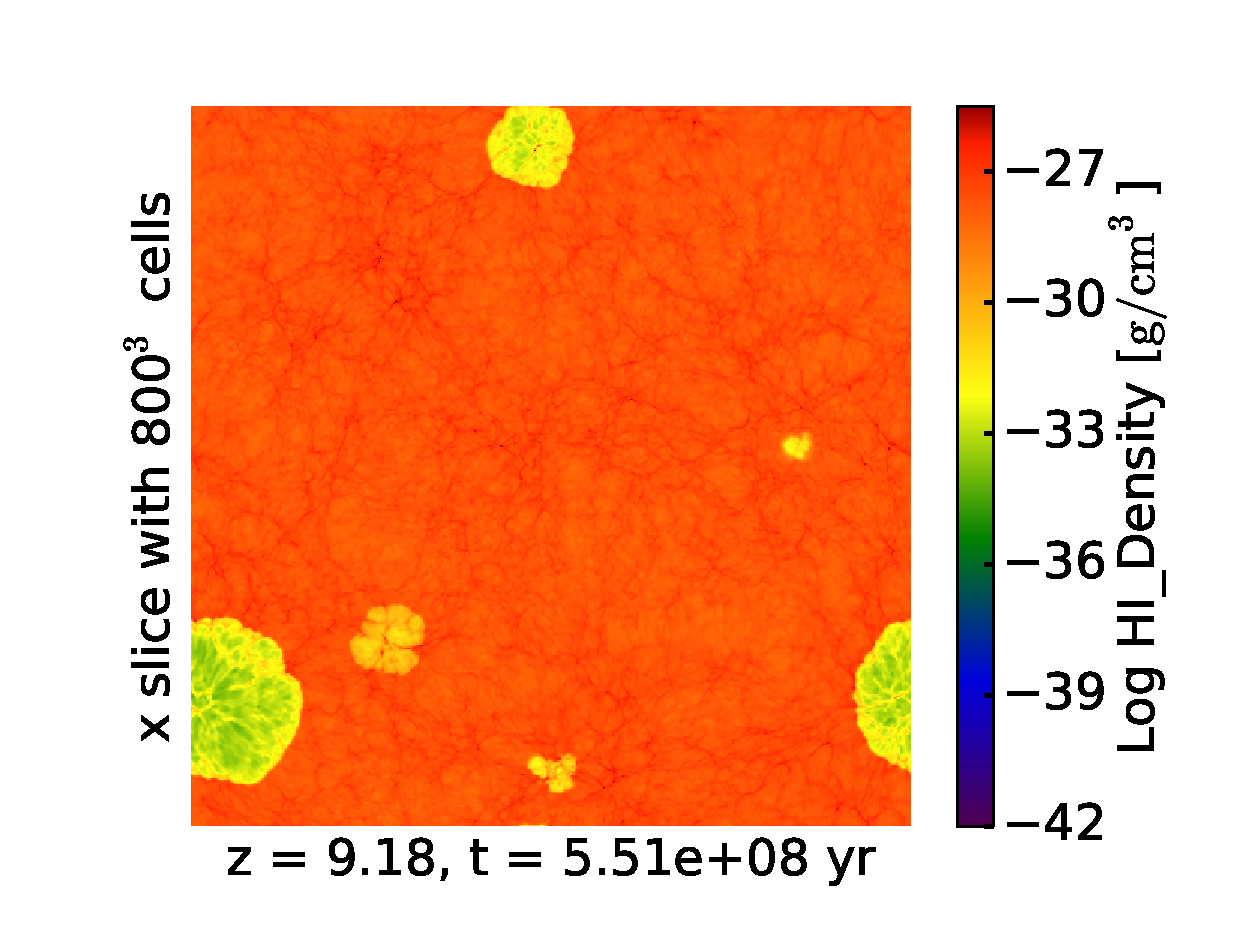
\includegraphics[trim = 15mm 5mm 0mm 15mm, clip, width=1.0\textwidth]{1_1_slice_HI_Density_x_HD4050.eps}
    \end{minipage}
\hspace*{-4.00mm}
    \begin{minipage}[h]{0.5\linewidth}
        \centering
        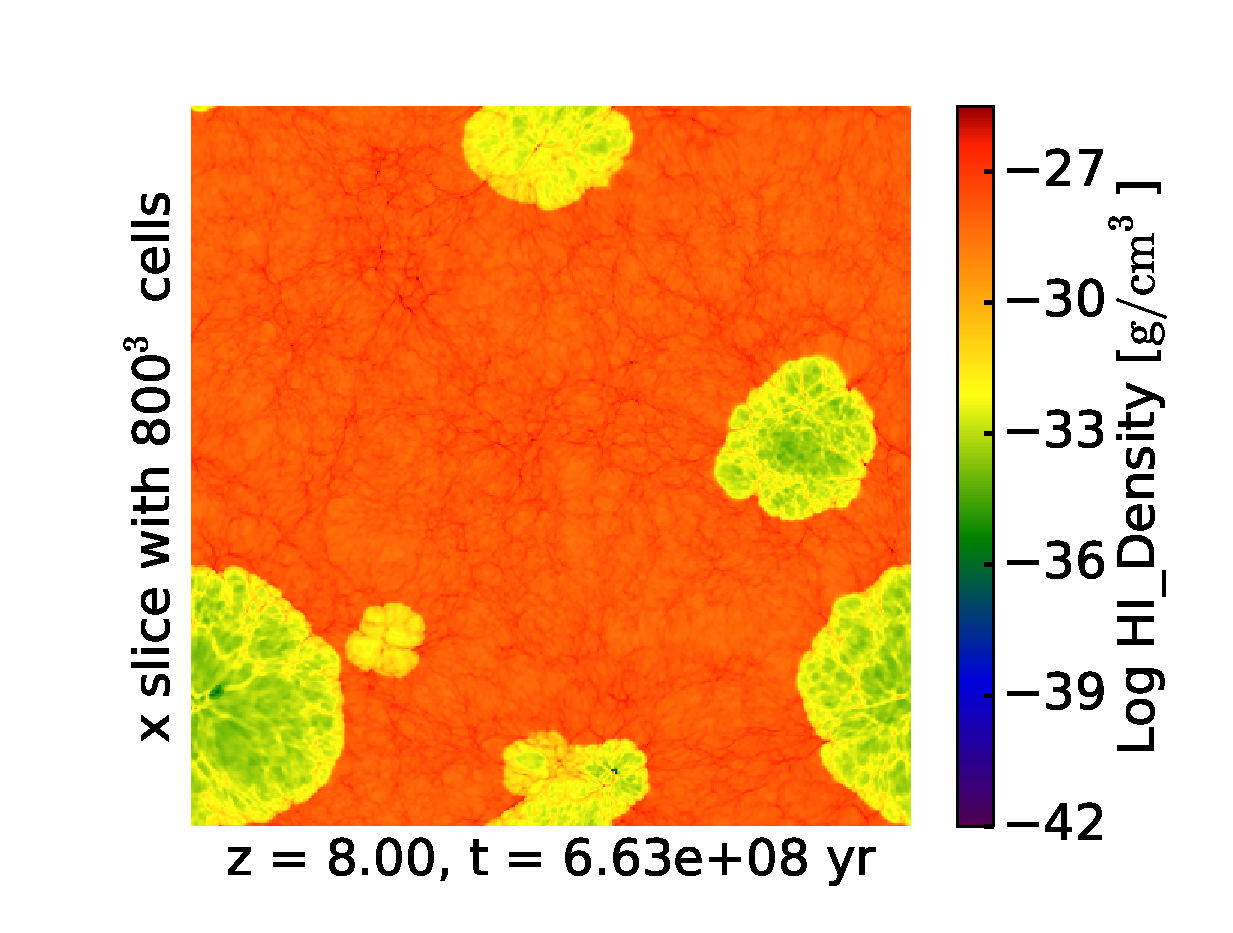
\includegraphics[trim = 15mm 5mm 0mm 15mm, clip, width=1.0\textwidth]{1_2_slice_HI_Density_x_HD6150.eps}
    \end{minipage}
\\
    \begin{minipage}[h]{0.5\linewidth}
        \centering
        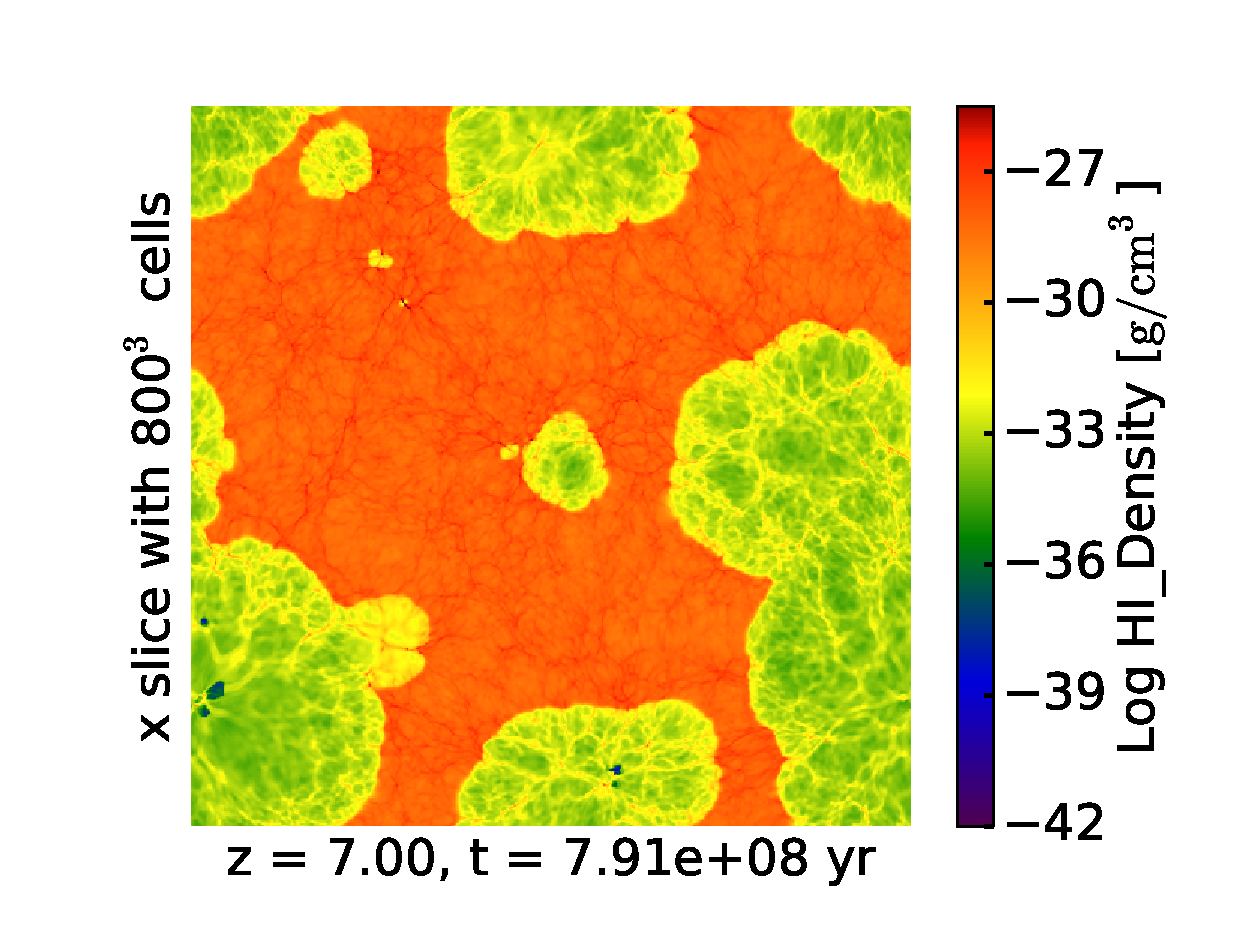
\includegraphics[trim = 15mm 5mm 0mm 15mm, clip, width=1.0\textwidth]{2_1_slice_HI_Density_x_HD7900.eps}
    \end{minipage}
\hspace*{-4.00mm}
    \begin{minipage}[h]{0.5\linewidth}
        \centering
        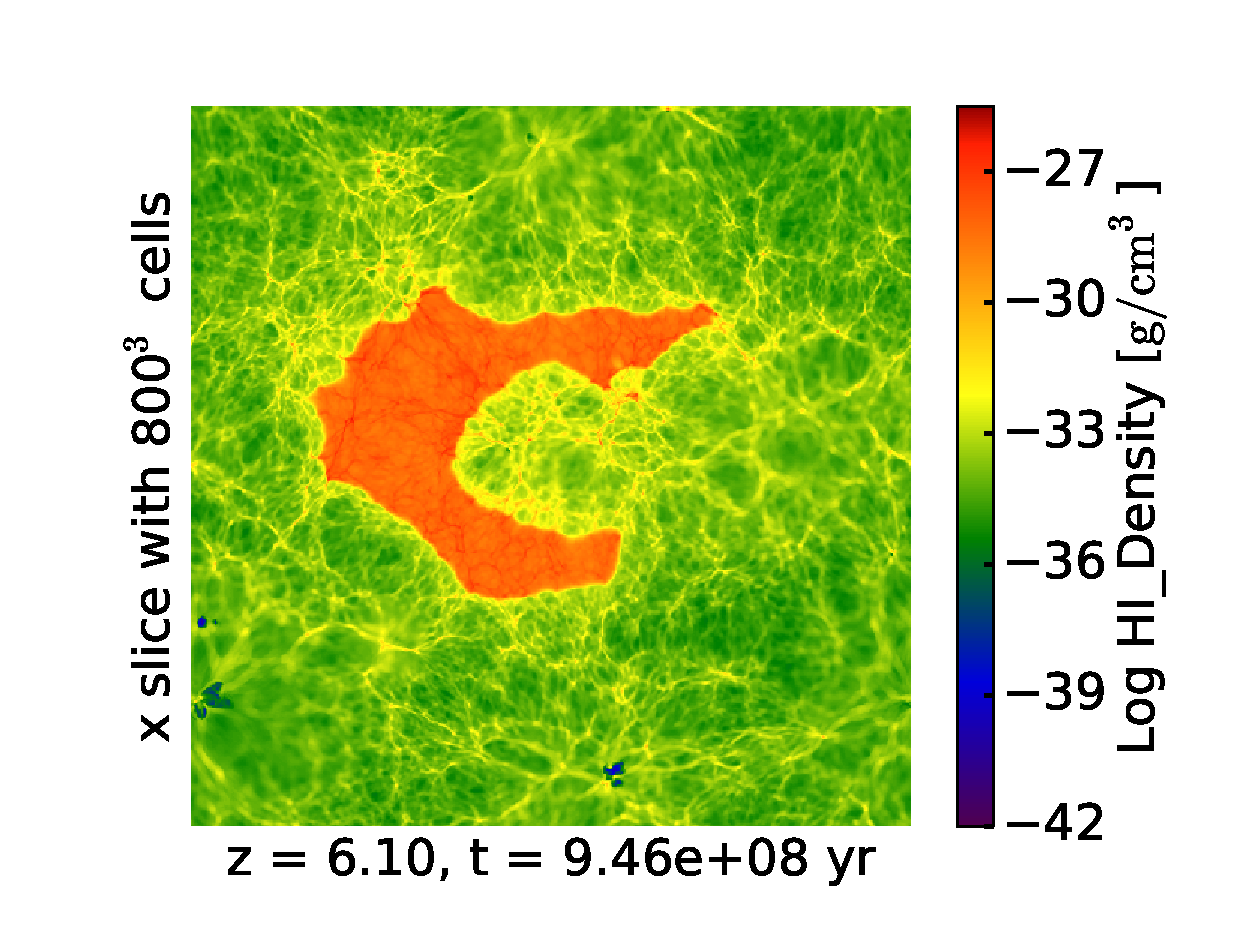
\includegraphics[trim = 15mm 5mm 0mm 15mm, clip, width=1.0\textwidth]{2_2_slice_HI_Density_x_HD14475.eps}
    \end{minipage}
    \caption{H {\footnotesize I} density on slices through the 20 Mpc volume showing the growth, 
percolation, and final overlap of H II regions. Panels show $z=9.18, 8.0,
7.0, 6.1$. The box becomes fully ionized at $z=5.8$ as the last neutral islands
are overrun by the I-fronts. Regions of extremely low H {\footnotesize I} density are shock-heated 
bubbles due to supernova feedback.}
    \label{HI_slices}
\end{figure*}

Here we first present the basic properties of the simulation before delving into specific topics in subsequent sections. The star formation and feedback parameters for this simulation are $f_* =0.1, f_{m*}=0.25, \epsilon_{SN}=10^{-5}, \epsilon_{UV}=1.38 \times 10^{-4}$. Figure \ref{HI_slices} shows the reionization process as it proceeds through growth, percolation, and final overlap of ionized hydrogen (H {\footnotesize II}) regions driven by ionizing radiation from star forming galaxies. We plot the neutral hydrogen (H {\footnotesize I}) density on a slice through the densest cell in the volume at redshifts $z=9.18, 8.0, 7.0, 6.1$.  At $z=9.18$ several isolated quasi-spherical I-fronts are intersected by the slice plane.  These grow and have begun to merge by $z=8.0$. By $z=7.0$ the toplogy is beginning to invert, in that there are now isolated peninsula of H {\footnotesize I} gas embedded in an otherwise ionized IGM. By $z=6.1$ the remaining neutral island has almost disappeared as it is being irradiated from all sides. We can also see in the figure small patches of extremely low H {\footnotesize I} density; these correspond to bubbles of shock heated gas near galaxies heated to above $10^6$K in temperature by supernova feedback.

\begin{figure}
	\includegraphics[width=0.5\textwidth]{E3Ionized_vs_Redshift.eps}
	\caption{Evolution of the ionized volume fraction versus redshift for hydrogen ionized to less than 1 neutral in 10$^3$ atoms.  As redshift decreases, the volume filling fraction grows rapidly until around redshift of 6, at which time the rate of growth slows significantly as the last neutral island is ionized .  The sensitivity of this curve to ionization level is discussed in \S\ref{QuantitativeLanguage}.}
	\label{Ion1E3}
\end{figure}

Figure \ref{Ion1E3} plots the evolution of the ionized volume fraction $Q_\mathrm{H\,II}$ versus redshift. Here a cell is called ionized if $\rho_\mathrm{H\,II}/\rho_\mathrm{H} \geq 0.999$ (In \S\ref{QuantitativeLanguage} we discuss the sensitivity of this curve to level of ionization.) The first ionizing sources turn on at $z \sim 10$ in this simulation. The ionized volume fraction rises rapidly, reaching 0.5 at $z \approx 6.8$, 0.95 at $z \approx 6.0$, and near unity at $z \approx 5.8$. We compare this evolution with the predictions of the simple analytic model introduced by \cite{MadauEtAl1999} in \S\ref{Qdot}. For now we only draw attention to the flattening of the curve in the redshift interval $5.8 \leq z \leq 6$. This is the signature of neutral islands being ionized by I-fronts converging in 3D, as opposed to being ionized by internal sources. 

Our simulation was not designed to complete reionization by a certain fiducial redshift. Rather we adjusted our star formation efficiency parameter $f_*$ so that we can approximately match the star formation rate density (SFRD) in \citep{BouwensEtAl2011}.  Our SFRD is shown in Figure \ref{SFR}, along with the Bouwens data, plotted without error bars. For reference we also include the fitting function described in \citep{HaardtMadau2012}.  This shows that our simulated universe is one that produces approximately the same amount of stars in a given comoving volume, albeit a bit low relative to the data. We also note that the SFRD begins to flatten out at $z \approx 6.5$, and even turns over after overlap at $z \approx 5.8$, rather than continue to rise as indicated by the data points.  This is an artifact of the small box size as a simulation completed in a 80 Mpc comoving on a side box with identical physics, mass, and spatial resolution and star formation/feedback parameters does not show this slowing down of the SFRD. This will be reported on in a future paper. 

\begin{figure}
	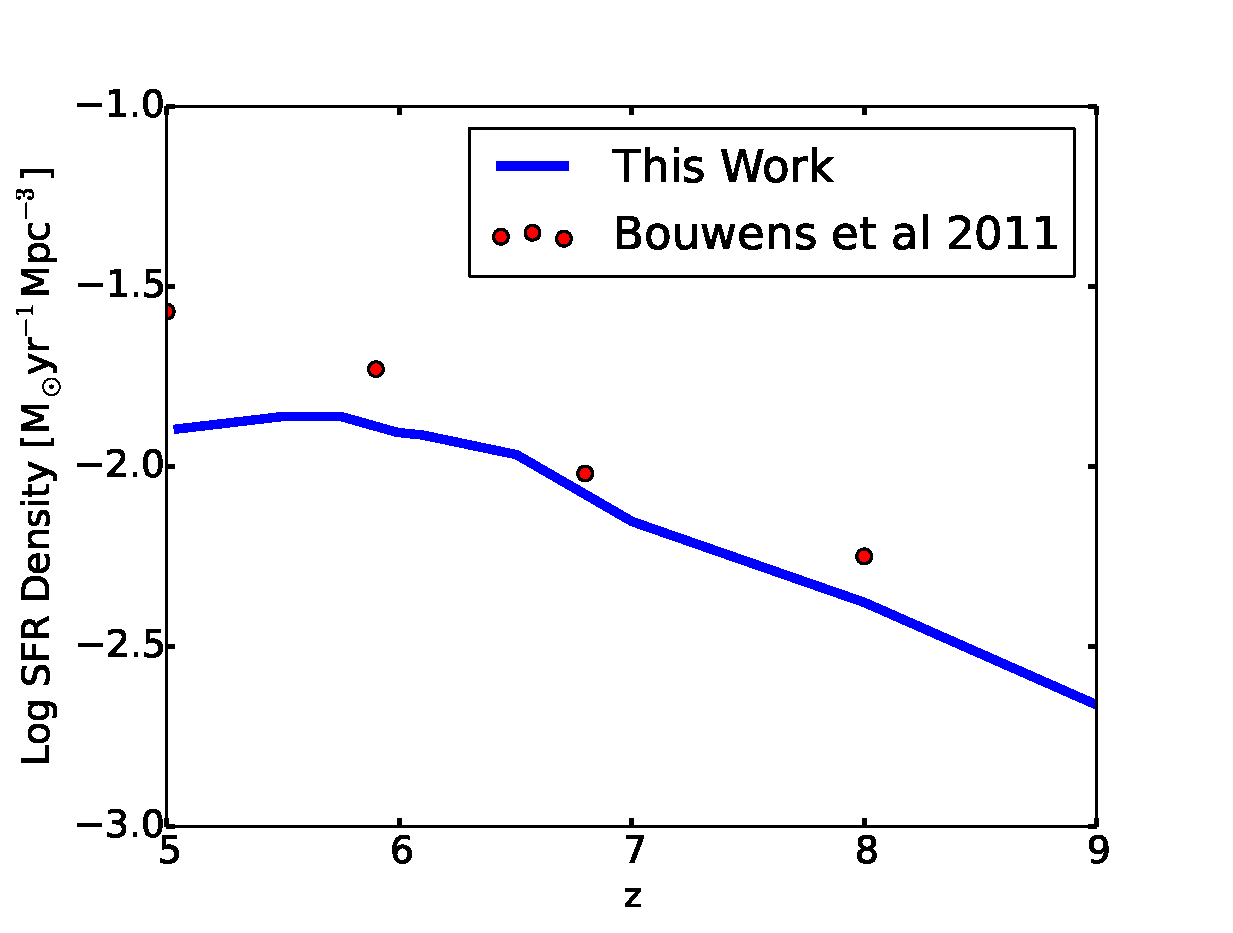
\includegraphics[width=0.5\textwidth]{compareSFR_haardt_madau2012.eps}
	\caption{A comparison of simulated and observed star formation rate densities (SFRD) in units of M$_\odot$yr$^{-1}$Mpc$^{-3}$ comoving.  Blue curve labeled ``This Work'' is from our 20 Mpc / $800^3$ simulation, and ``Bouwens et al 2011'' are observationally derived data points from \cite{BouwensEtAl2011b} plotted without error bars. The leveling off of the simulated SFRD is an artifact of the small volume as a simulation carried out with identical physics, mass, and spatial resolution but in 64 times the volume does not show this effect.}
	\label{SFR}
\end{figure}

%Another general feature of the simulation is how fast the universe is reionized.  We look at a %specific ionization level (less than 1 neutral hydrogen in 10$^3$ hydrogen), and plot its volume %filling fraction versus redshift.  We shall discuss in depth what happens when we look at a range %of different ionization levels in \S\ref{QuantitativeLanguage}, but for now, consider the cell in %the simulation as ``completely'' ionized when it reaches this ionization state.  Figure %\ref{Ion1E3} shows in linear scale that the universe has slightly more than 10\% of its volume %completely ionized at a redshift of 8, and by a redshift of 6, more than 90\% of the volume is %completely ionized.

%One should note that the rate at which the volume filling fraction curve rises with respect to %decreasing redshift slows down significantly near redshift of 6.  This is an artifact of the way %radiation and ionization front is transported.  As the last region of space that is left mostly %neutral, it faces incoming ionization radiation waves from all sides.  Since the waves are %converging in 3 dimensions, the amount of H {\footnotesize I} volume that is swept through %with each unit of time gets smaller and smaller.  Although the propagation of the wave fronts %may not be exactly constant and the x axis of redshift is not exactly the same as time, the %analogy holds true.



To check and make sure that our simulation is giving us a fair representation of the universe, we plot several more quantities and look for any anomalies.  In Figure \ref{HMF}, we see that our halo mass function at redshift of $z \sim 6$ matches well with the Warren fit implemented in \texttt{yt} \citep{WarrenEtAl2006,TurkEtAl2011}.  The mass function captures haloes down to $\sim$10$^8$M$_\odot$, which as previously stated was a simulation design criterion.  The haloes are found by first running the parallelHOP halo finder installed in \texttt{yt} \citep{SkoryEtAl2010}, then taking the linked list of dark matter particles for each halo and wrapping the region around them in an ellipsoidal 3D container introduced in \texttt{yt} 2.4.  The 3D container enables the query of the fluid quantities of the haloes, such as baryonic, emissivity, radiation contents in addition to the particle information.  Since the dark matter particles used are $\sim 5 \times$ 10$^5$M$_\odot$, the 10$^8$M$_\odot$ dark matter haloes are considered to be resolved \citep{TrentiEtAl2010}.

\begin{figure}
	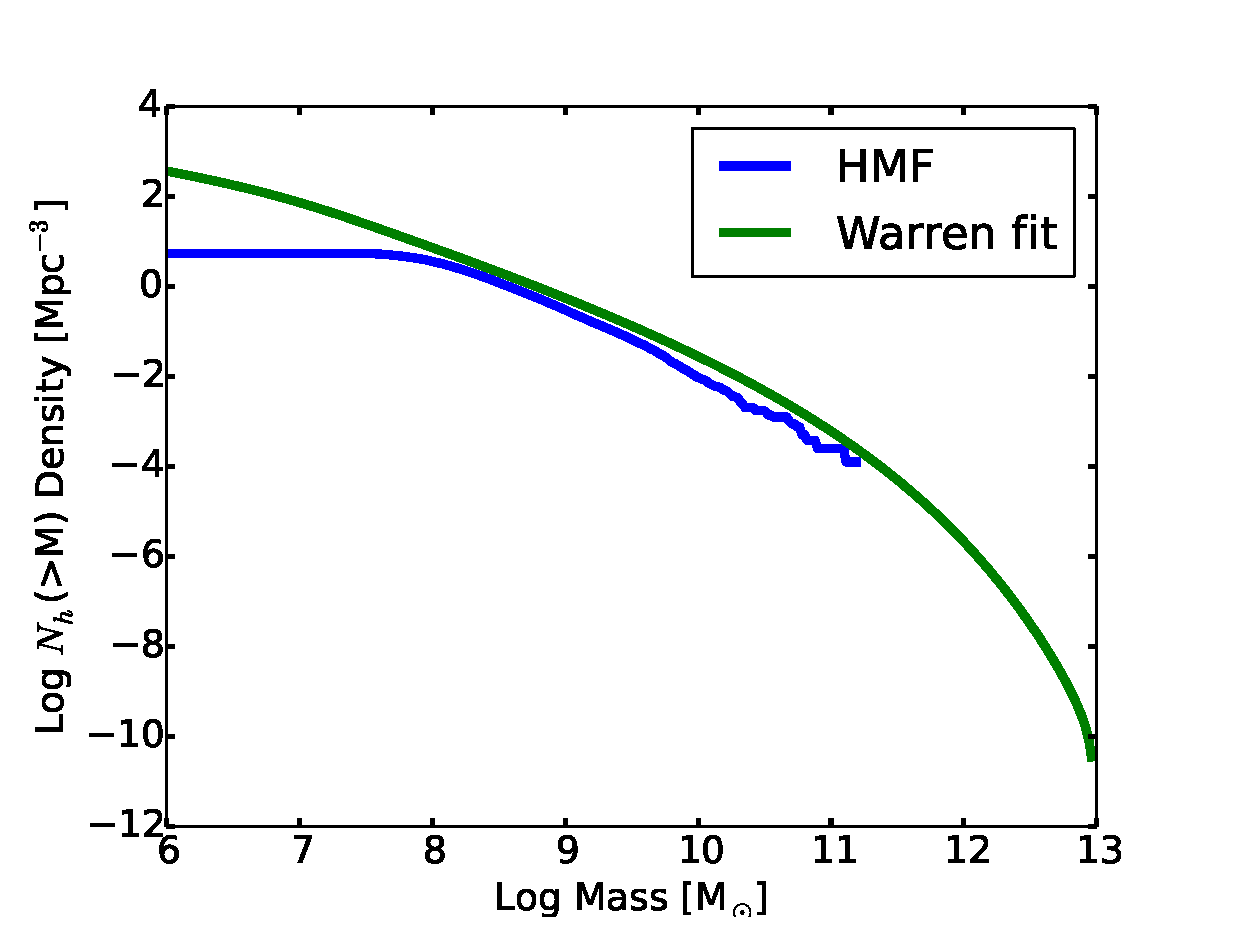
\includegraphics[width=0.5\textwidth]{HD14475_HMF.eps}
	\caption{The dark matter halo mass function from our simulation (blue line).  Green line is the fit from \citep{WarrenEtAl2006}. Our low-mass HMF is reasonably complete down to $M_{halo} \approx 10^8 M_{\odot}$; i.e. halos believed to form stars efficiently due to atomic line cooling. Incompleteness at the high mass end is due to the limited volume sampled.}
	\label{HMF}
\end{figure}

As a final check that our ionizing source population is not wildly unrepresentative of the observed universe, in Figure \ref{scaledLF} we plot the luminosity function of our simulated galaxies at $z=6.1$ along side the observational data points from Table 5 of \citep{BouwensEtAl2007}. The points in red are the bolometric luminosities for our galaxy population calculated directly from the $z=6.1$ halo catalogue.  To calculate the luminosity of a given halo we sum the emissivity field within the 3D ellipsoidal containers defined by the halos' dark matter particles.  Our error bars are taken using one standard deviation of luminosity in the mass bins.  Although this is not proof that our simulation is matching observations exactly, it does lend support that our realization of reionization is being driven by sources not too dissimilar to those observed and is sufficient for the purposes of this study. 

\begin{figure}
	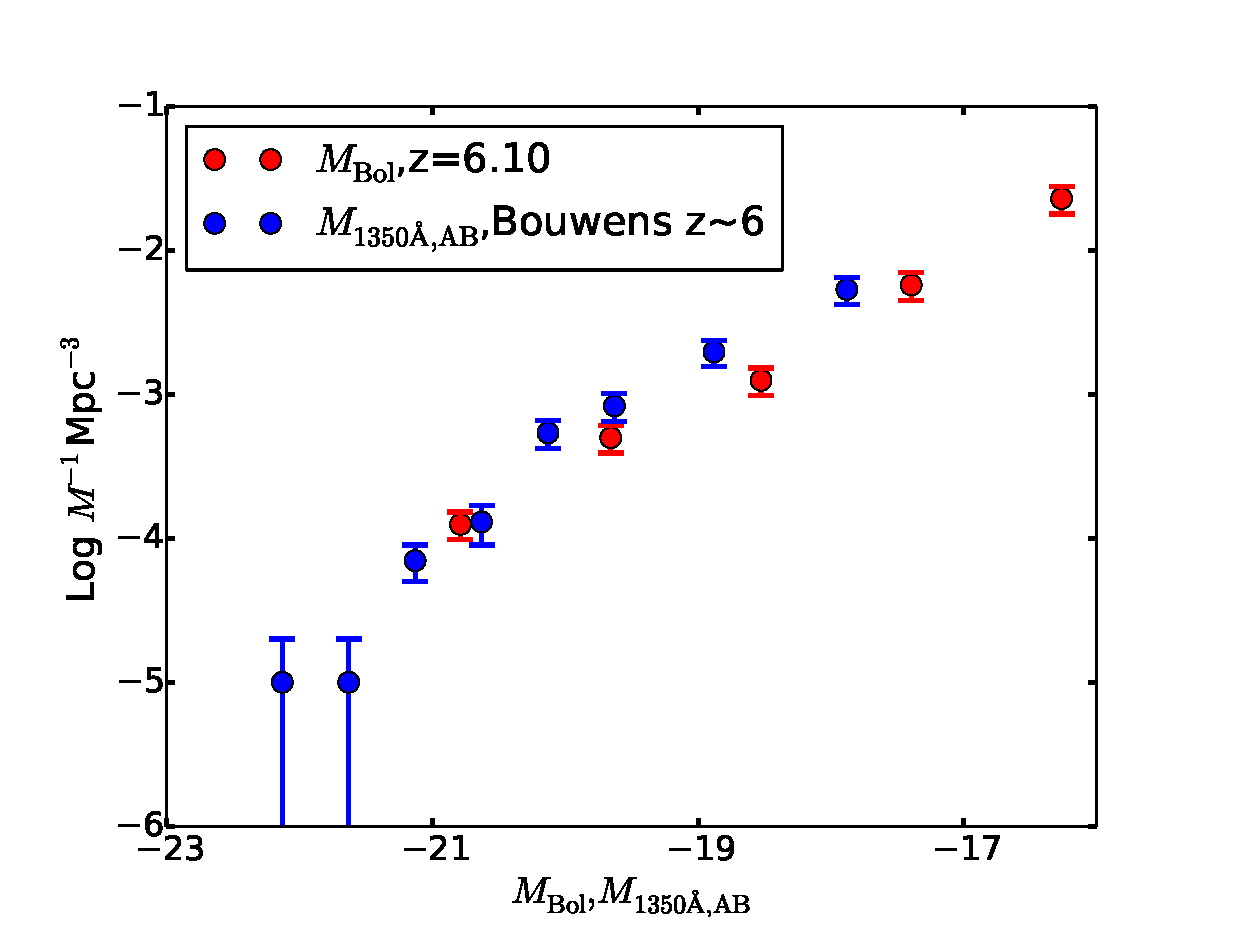
\includegraphics[width=0.5\textwidth]{scaledLF.eps}
	\caption{Bolometric luminosity function derived from our simulation data (red), compared with observational data points (blue) from \citep{BouwensEtAl2007}.}
	\label{scaledLF}
\end{figure}

\subsection{Quantitative Language}
\label{QuantitativeLanguage}

Earlier works on reionization such as \cite{ValageasSilk1999,Gnedin2000,MiraldaEscudeEtAl2000,IlievEtAl2006} speak of a two phase medium composed of completely neutral and completely ionized hydrogen gas, while more recent works \citep{CiardiEtAl2003,ZahnEtAl2007,ShinEtAl2008,PetkovaSpringel2011a,FinlatorEtAl2012} begin to consider the {\em degree of ionization} within ionized gas.  The simplification of considering a two phase medium helps reduce the simulation complexity and the language needed to describe the results.  However, as simulations become more sophisticated, the two phase paradigm becomes ill-suited to convey the wealth of information contained in the larger and more detailed simulations.  
As people begin to describe the new simulations, the old paradigm lingers and causes ambiguities. As a case in point, consider the ionized volume filling fraction versus redshift, one of the simplest quantitative metrics of any reionization simulation. Within the framework of a two-phase medium, this is uniquely defined at any redshift. For a simulation such as ours which tracks the ionization state in every cell, the volume filling fraction depends on the degree of ionization, as illustrated in Figure \ref{linearIonized}. 

%From the earliest N-body simulations to simulations with baryonic fluids to different ionization states of these quantities, simulations have made %big strides in terms of complexity.  If the language we use to describe the ionization state stagnates at distinguising only between two phases %using a single threshold, then we neglect the spectrum of information from the simulation.  This is why we propose that the community come up %with a more unified and quantitative way to describe the simulations.  For that end, we will try to raise two areas where this is apparent.

%As alluded to earlier in \S\ref{GeneralAspects}, we now investigate the ionization volume filling fraction more thoroughly.  When we plot other %ionization levels and their volume filling fraction versus redshift, the result is Figure \ref{linearIonized}.  
This figure shows the evolution of the volume filling fraction of ionized gas which exceeds a minimum local ionization fraction $f_i \equiv \rho_\mathrm{H\,II}/\rho_\mathrm{H}$. The three thresholds are $f_i=$ 0.1, 0.999, and 0.99999 and are labelled 10\%, 1E3, 1E5, respectively in Figure \ref{linearIonized}. 
We choose three specific levels not because we think they are more important than others, but because it suits our later narrative and gives a range values.  With the ionization state tracked by the simulation, we see that it is now ambiguous to ask at what redshift 50\% of the volume is ionized. In our simulation this occurs at $z \approx$ 7, 6.8 and 6.5 for $f_i$=0.1, 0.999, and 0.99999, respectively.

%We choose these numbers to demonstrate what can be done, but the values themselves are in no way set in stone.  The figure shows 10\% %ionization (having more than 1 ionized hydrogen per 10 hydrogen atoms), 1E3 (having less than 1 neutral hydrogen per 10$^3$ hydrogen atoms), %and 1E5 (having less than 1 neutral hydrogen per 10$^5$ hydrogen atoms), their volume filling fraction versus redshift.  In Figure %\ref{LogIonized}, the same information is plotted with the y-axis in Log$_{10}$ scale.

\begin{figure}
	\includegraphics[width=0.5\textwidth]{Ionized_vs_Redshift.eps}
	\includegraphics[width=0.5\textwidth]{Log_Ionized_vs_Redshift.eps}
	\caption{Volume filling fraction of ionized gas versus redshift for three ionized fraction thresholds. {\em Top} linscale; {\em Bottom} logscale. The three ionization levels are ``10\%'' in blue: fractional volume that have more than 1 ionized hydrogen atom per 10 hydrogen atoms.  ``1E3'' in green: fractional volume that have less than 1 neutral hydrogen atom per 10$^3$ hydrogen atoms.  ``1E5'' in red:  fractional volume that have less than 1neutral hydrogen atom per 10$^5$ hydrogen atoms.}
	\label{linearIonized}
\end{figure}

%\begin{figure}
% 	\includegraphics[width=0.5\textwidth]{Log_Ionized_vs_Redshift.eps}
%	\caption{Plot of the same information as Figure \ref{linearIonized}, however, this time theh y-axis is in Log$_{10}$ scale}
%	\label{LogIonized}
%\end{figure}


%One key element is that one should always talk about the level of ionization, and not throw around terms like ``ionized'' lightly, unless %predefined.  For example, we can tell when 10\% of the universe's volume is at a ionization level of 10\%.  This occurs around a redshift of 8.7 %(estimates are from simple linear interpolation of the available data output intervals).  Studying another curve, we see that 10\% of the universe's %volume is ionized to 1E5 around a redshift of 7.7.  

In the rest of this paper we will often report results as a function of these three ionization fraction thresholds. 
To make the text easier to read we will use the terms ``Ionized'' to designate $f_i$=0.1, ``Well Ionized'' to designate $f_i$=0.999, and ``Fully Ionized'' to designate $f_i$=0.99999 ionization levels.
%This graph ultimately shows that more of the universe becomes more highly ionized as redshift decreases.  Also, it is harder to make claims about %the ``entire'' universe having reached a specific ionization level, because there's often regions that may not have reached a specific level.

\subsection{Inside-out or Outside-in}
\label{IOOI}

Besides specifying the amount of ionized volume and levels of ionization, another area where quantitative language is useful is in the description of the reionization history.  Since the Outside-in model was proposed by \cite{MiraldaEscudeEtAl2000}, there is gathering support for the opposing view of the Inside-out model by \cite{SokasianEtAl2003,FurlanettoEtAl2004,IlievEtAl2006} to name a few.  In \cite{FinlatorEtAl2009}, the authors go even further and add to the lexicon ``Inside-outside-middle'', trying to describe the rich detail in a reionization scenario. The basic Inside-out picture is that galaxies form in the peaks of the dark matter density field and drive expanding H {\footnotesize II} regions into their surroundings ({\em expansion phase}). 
%by virtue of the UV radiation emitted from young, massive stars. 
These H {\footnotesize II} regions are initially isolated, but begin to merge into larger, Mpc-scale H {\footnotesize II} regions due to the clustering of the galaxy distribution ({\em percolation phase}). Driven by a steadily increasing global star formation rate and recombination time (due to cosmic expansion) this process goes on until H {\footnotesize II} regions completely fill the volume ({\em overlap phase}). In this picture, rare peaks in the density field ionize first while regions of lower density ionize later from local sources that themselves formed later. 


To investigate how reionization progresses in regions of different density, we plot in Figure \ref{NeutralPhase} the hydrogen neutral fraction ($\rho_\mathrm{H\,I}/\rho_\mathrm{H}$) versus overdensity $\Delta_b\equiv\rho_b/\langle\rho_b\rangle$ in the left column, and in the right column a slice of the gas temperature, with redshift decreasing from top to bottom.  One would expect if inside-out ionization is the case, that the neutral fraction of higher density region should drop down more quickly than lower density regions.  Below, we will describe each row of the figure in more detail.

Looking at the redshift $z=10$ row, we see in the gas temperature slice that two isolated regions of ionization appear due to UV feedback from new stars, indicated by the $\sim$10$^4$K gas . These regions correspond to places on the neutral fraction vs. overdensity phase plot where a small amount of volume emerges around $\Delta_b$ of $10^{-1}-10^1$, reaching Well Ionized to Fully Ionized levels.  The T $\sim$10$^7$K region corresponds to the extended tail of very low neutral fraction gas in the left column, and indicates gas shock heated by supernova feedback.  Although the cell count of shock heated gas will grow, it remains orders of magnitude smaller compared to the photoionized regions that we will emphasize.  Even at this early stage, there are high density regions above $\Delta_b$ of 10$^2$-10$^3$ that are Well Ionized; this is due to their close proximity to the ionizing sources, supporting the Inside-out paradigm.

Looking at the next row of figures at a redshift of $z=7$, we see that the volume of Well Ionized regions has increased greatly, and so has the shock heated region in the phase plot.  We also see that most, but not all the $\Delta_b > 10^2$ cells have reached the Well Ionized level.  Although a large portion of the volume is in the Well Ionized regime, the majority of the volume (the red pixels) is still neutral, as we can see in the corresponding temperature slice plot.  Most of the volume is still well under 10$^4$K, where we expect the temperature to hover around once the ionization front has passed through the region and the gas has had time to come into photoionization thermal eqilibrium. 

By a redshift of $z=6.1$, we see from the left column that the region that is ionized beyond the Fully Ionized level (an irony in terms, which means there is definitely room for improvement in the naming convention), dominates the simulation volume.  There are still some regions not yet consumed by the ionization front, that is seen on the top of the neutral fraction plot and on the right according to the temperature slice.

The next row at redshift of $z=5.5$ is after the entire volume has been swept over by ionization fronts.  Most of the volume is beyond the Well Ionized level, except for a few cells around $\Delta_b \sim 10^2$.  There are also some cells that are still neutral around $\Delta_b \sim 10^4$.  They remain neutral because their densities are so high, leading to high recombination rates.  Over time these cells will shift up and down the neutral fraction plot with waves of star formation and supernova explosions since they are likely close to the source of the radiation and kinetic energy.

The last row of Figure \ref{NeutralPhase} is at redshift $z\sim5$, where we can see that the previous few cells that have yet to reach Well Ionized levels around $\Delta_b \sim 10^2-10^3$ have now disappeared.  The cells that have not reached Well Ionized level before are cells where either the radiation is not strong enough due to shielding effects or the density is so high the gas recombines quickly even after being ionized.  After the ionization front has passed though and highly ionized the IGM, there is little material left to shield against the radiation background and we see all but the densest few cells become Well Ionized. The high density region reaching the same ionization level after the under dense void, would fit well with the description for the Outside-in model.  Note, that the remaining cells that finally reached Well Ionized levels, are orders of magnitude smaller in total volume compare to the rest of the cells at the same density.  So if we call cells of $\Delta_b \sim 10^2$ filaments, not all dense filaments get Well Ionized until late in the EoR.  Before the volume is filled with radiation, these dense filaments are able to remain relatively neutral.

Unfortunately, the evolution of these redshift panels is not enough to capture the propagation of radiation fronts from the initial sources, but they do convey the overall ionization history of the universe.  The panels suggest that the region surrounding the ionization sources, whether they are dense cores, filaments, or voids, are all affected by the radiation on roughly the same time scale.  However, the degree to which they are ionized is different.  It is this difference, that is the key to answering the original question, whether the universe ionize inside-out or outside-in.  

When focusing on the ionization of the IGM, lets for a moment neglect the $\Delta_b \sim10^4$ cells that shift ionization level with waves of star formation which comprise a tiny fraction of the volume.  If we use the ``Ionized'' level to characterize something as completely ionized and draw the line for neutral fraction at 10\%, then the universe reaches end of EoR before $z \sim 5.5$.  Since radiation propagates from sources outward, that would correspond to the Inside-out picture.  If we were to instead draw the completely ionized line at ``Well Ionized'' level, then we can see that even at $z \sim 5.5$, there is a small peak in the dense region of the phase diagram ($\Delta_b \sim 2.4\times10^2$) that has yet to reach below the line to be considered completely ionized.  This would correspond to the Outside-in picture which reaches end of EoR sometime before $z \sim 5$ (or Inside-outside-middle if one uses the \cite{FinlatorEtAl2009} terminology and considers the neutral peak to be a part of the filaments).  And finally, if we were to draw the line at the ``Fully Ionized'' level, the universe has yet to ionize even for regions that are only 10$\times$ over dense.  Thus the ionization history is a story with many perspectives, and it really depends on how the story teller draws the line as to whether Inside-out, Outside-in, or Inside-outside-middle is a better qualitative description. 

%To conclude this arduous and complex tale told by the few panels shown, is that reionization can be
%told with varying accuracy and focus.  The accuracy and focus can and will change the narrative that is finally distilled.  We would like to claim that the previous 
%authors all told a side of a story on this in, out, middle issue.  But, at the risk of sounding clich\'e, the whole story indeed is a combination of those pieces.  So, 
%unless we use the same quantitative language to describe these simulations, we may seem like disagreeing, while trying to tell a side of the same story.

%\begin{figure}
%	\includegraphics[width=0.7\textwidth]{color_phase_slice.png}
%	\caption{Left column: Plot of hydrogen neutral fraction versus over density with decreasing redshift from top to bottom.  Right column: Plot of Log temperature [K] projections through the simulation centered on a region that remained mostly neutral right before the ionization fronts engulf it at redshift of $\sim$6, with decreasing redshift from top to bottom.  Please refer to \S\ref{IOOI} for detailed description.}
%      \label{NeutralPhase}

%\end{figure}

\begin{figure*}[!tp]
	\begin{minipage}[h]{0.33\linewidth}
	\centering
	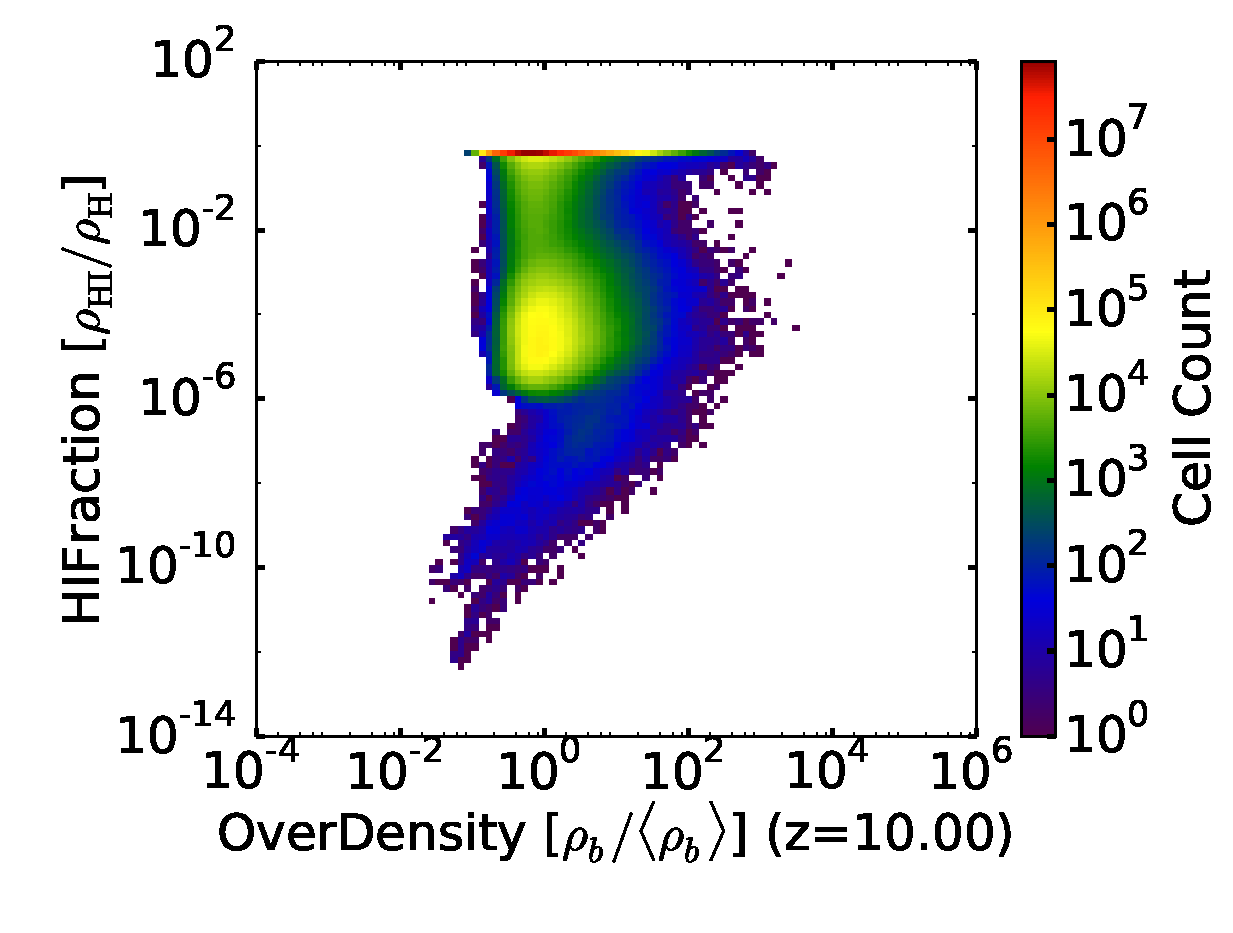
\includegraphics[trim = 7mm 9mm 1mm 7mm, clip, width=1.0\textwidth]{1_1_RD0029OverDensityHIFraction.eps}
	\end{minipage}
\hspace*{-2.00mm}
	\begin{minipage}[h]{0.33\linewidth}
	\centering
	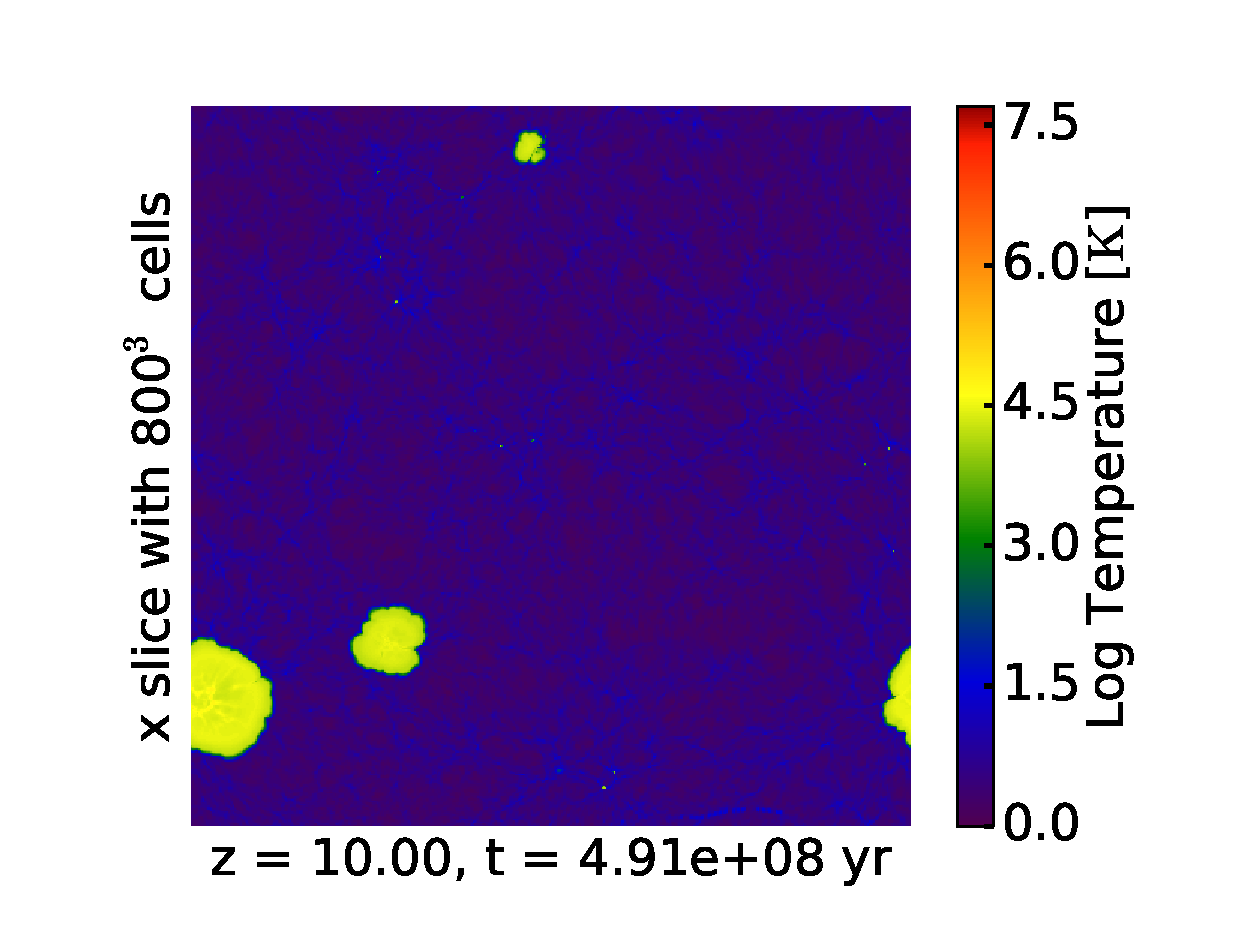
\includegraphics[trim = 10mm 0mm 7mm 7mm, clip, width=1.0\textwidth]{1_2_slice_Temperature_x_RD0029.eps}
	\end{minipage}
\hspace*{-2.00mm}
	\begin{minipage}[h]{0.33\linewidth}
	\centering
	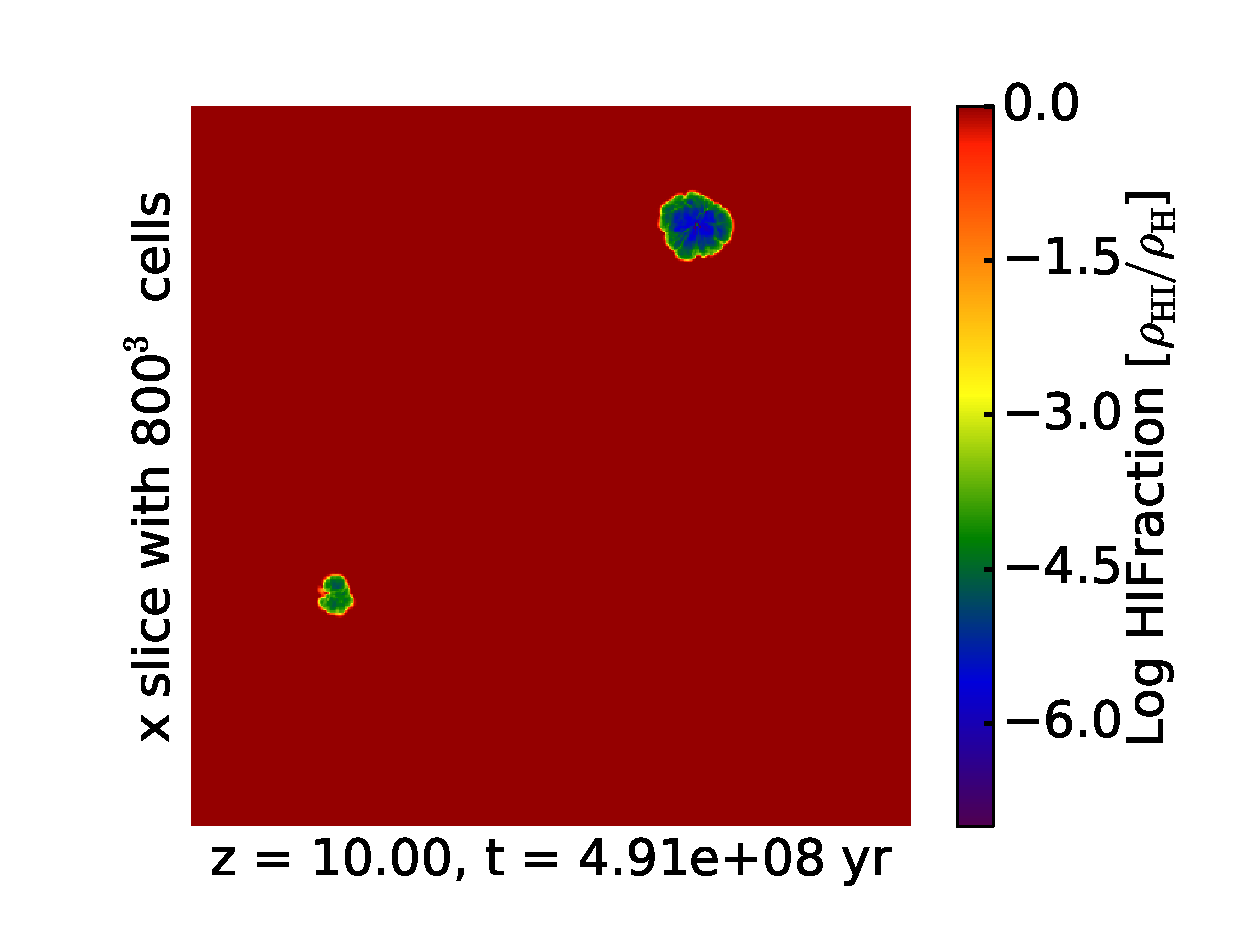
\includegraphics[trim = 10mm 0mm 7mm 7mm, clip, width=1.0\textwidth]{1_3_slice_HIFraction_x_RD0029.eps}
	\end{minipage}
\vspace*{-2.00mm}\\
	\begin{minipage}[h]{0.33\linewidth}
	\centering
	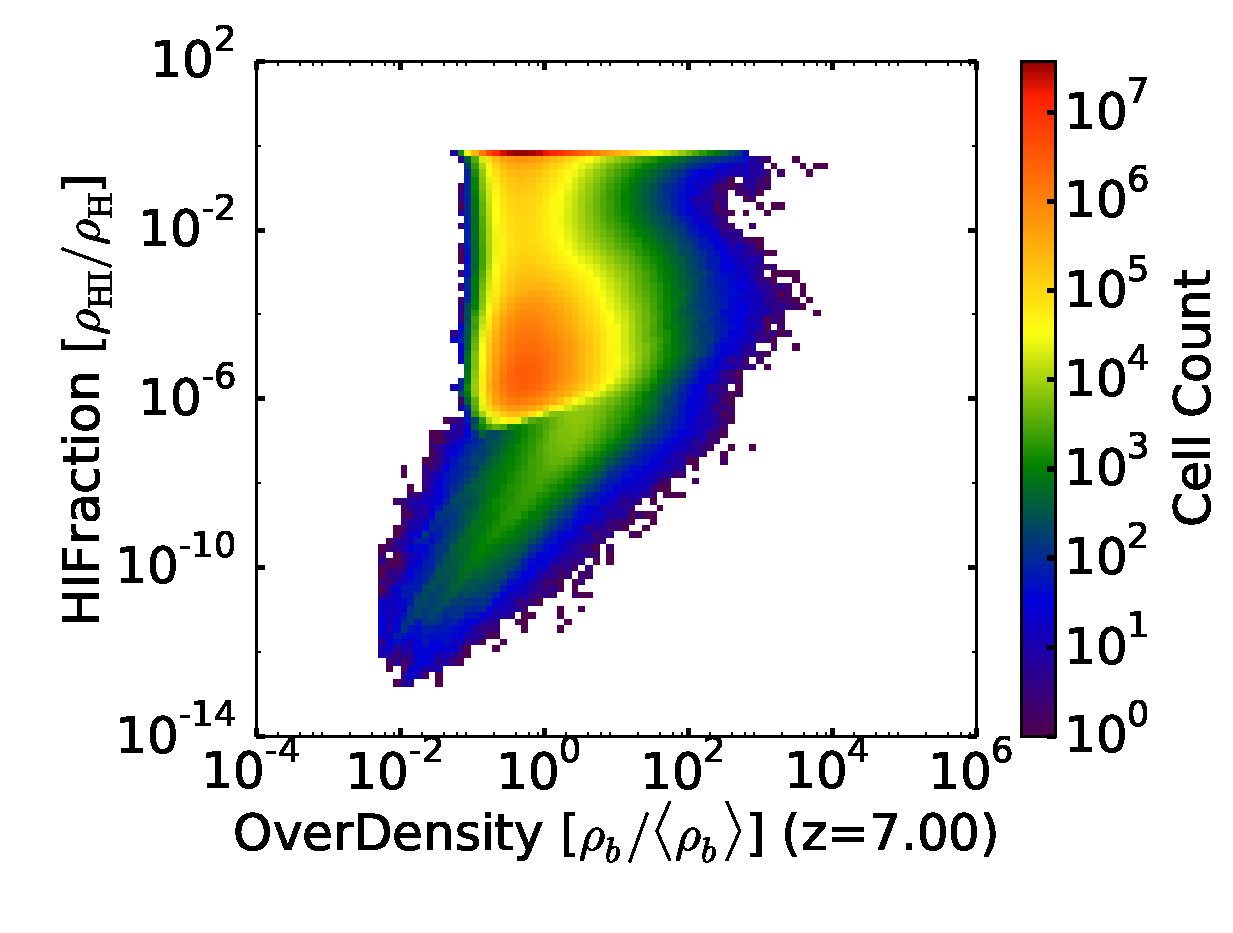
\includegraphics[trim = 7mm 9mm 1mm 7mm, clip, width=1.0\textwidth]{2_1_HD7900OverDensityHIFraction.eps}
	\end{minipage}
\hspace*{-2.00mm}
	\begin{minipage}[h]{0.33\linewidth}
	\centering
	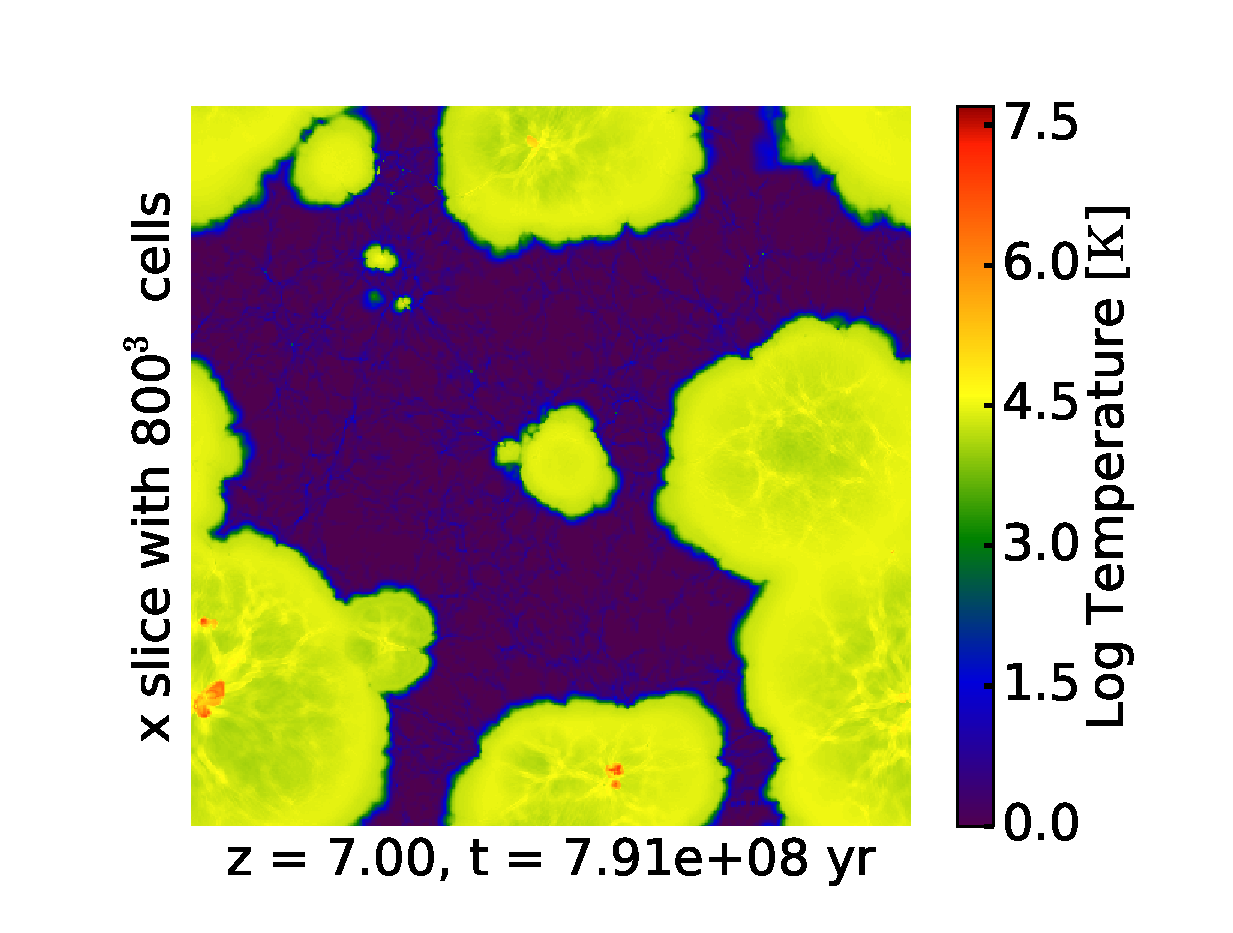
\includegraphics[trim = 10mm 0mm 7mm 7mm, clip, width=1.0\textwidth]{2_2_slice_Temperature_x_HD7900.eps}
	\end{minipage}
\hspace*{-2.00mm}
	\begin{minipage}[h]{0.33\linewidth}
	\centering
	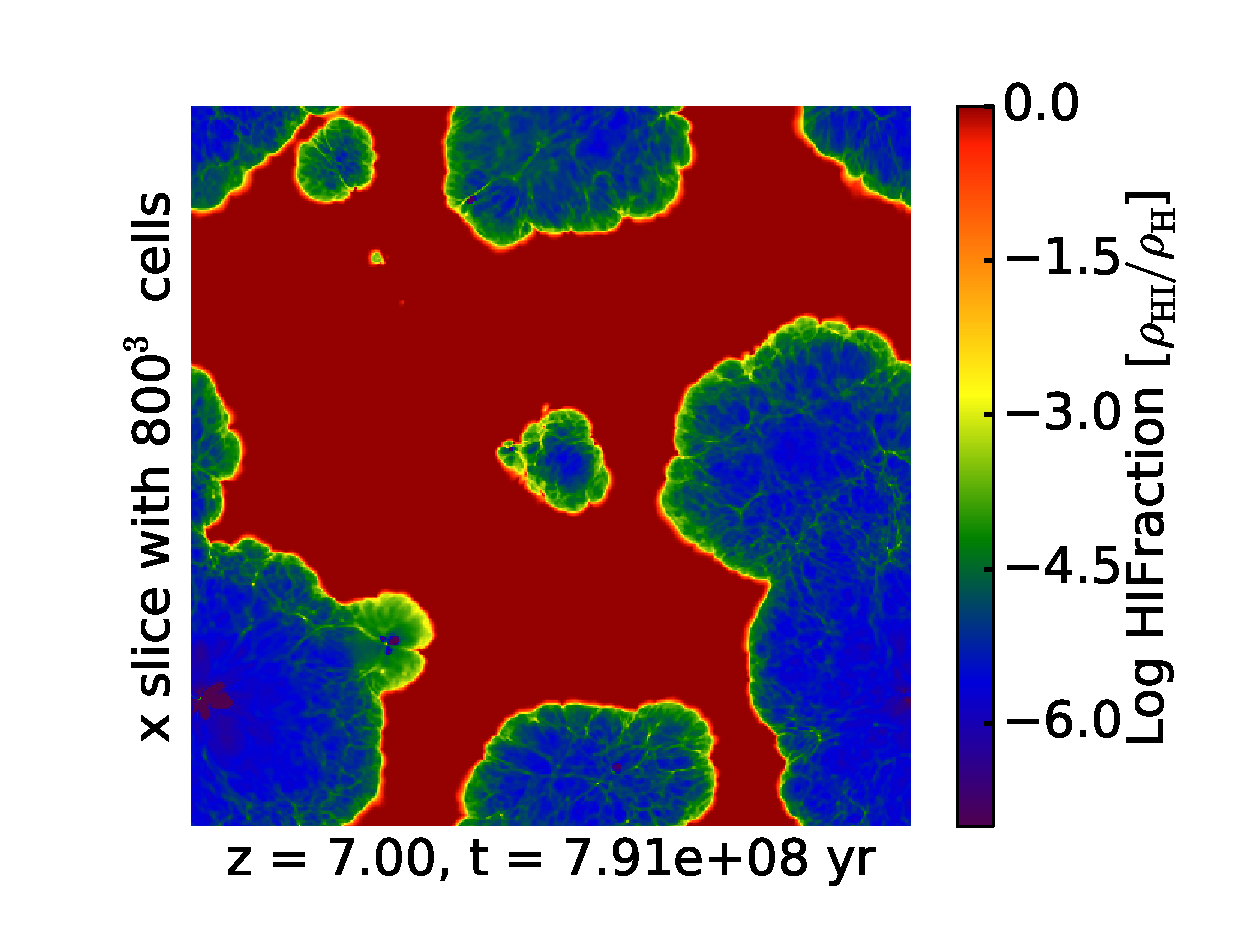
\includegraphics[trim = 10mm 0mm 7mm 7mm, clip, width=1.0\textwidth]{2_3_slice_HIFraction_x_HD7900.eps}
	\end{minipage}
\vspace*{-2.00mm}\\
	\begin{minipage}[h]{0.33\linewidth}
	\centering
	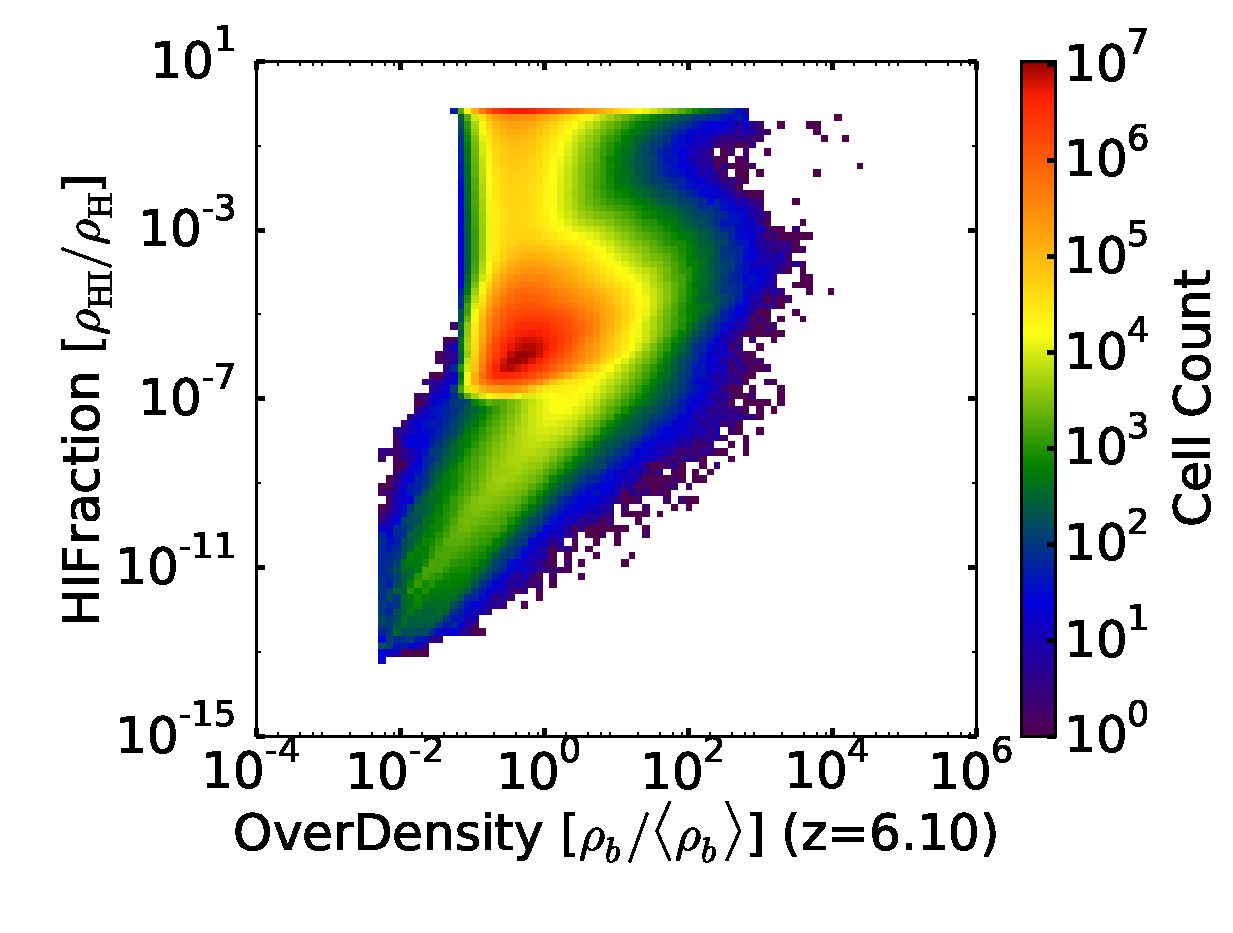
\includegraphics[trim = 7mm 9mm 1mm 7mm, clip, width=1.0\textwidth]{3_1_HD14475OverDensityHIFraction.eps}
	\end{minipage}
\hspace*{-2.00mm}
	\begin{minipage}[h]{0.33\linewidth}
	\centering
	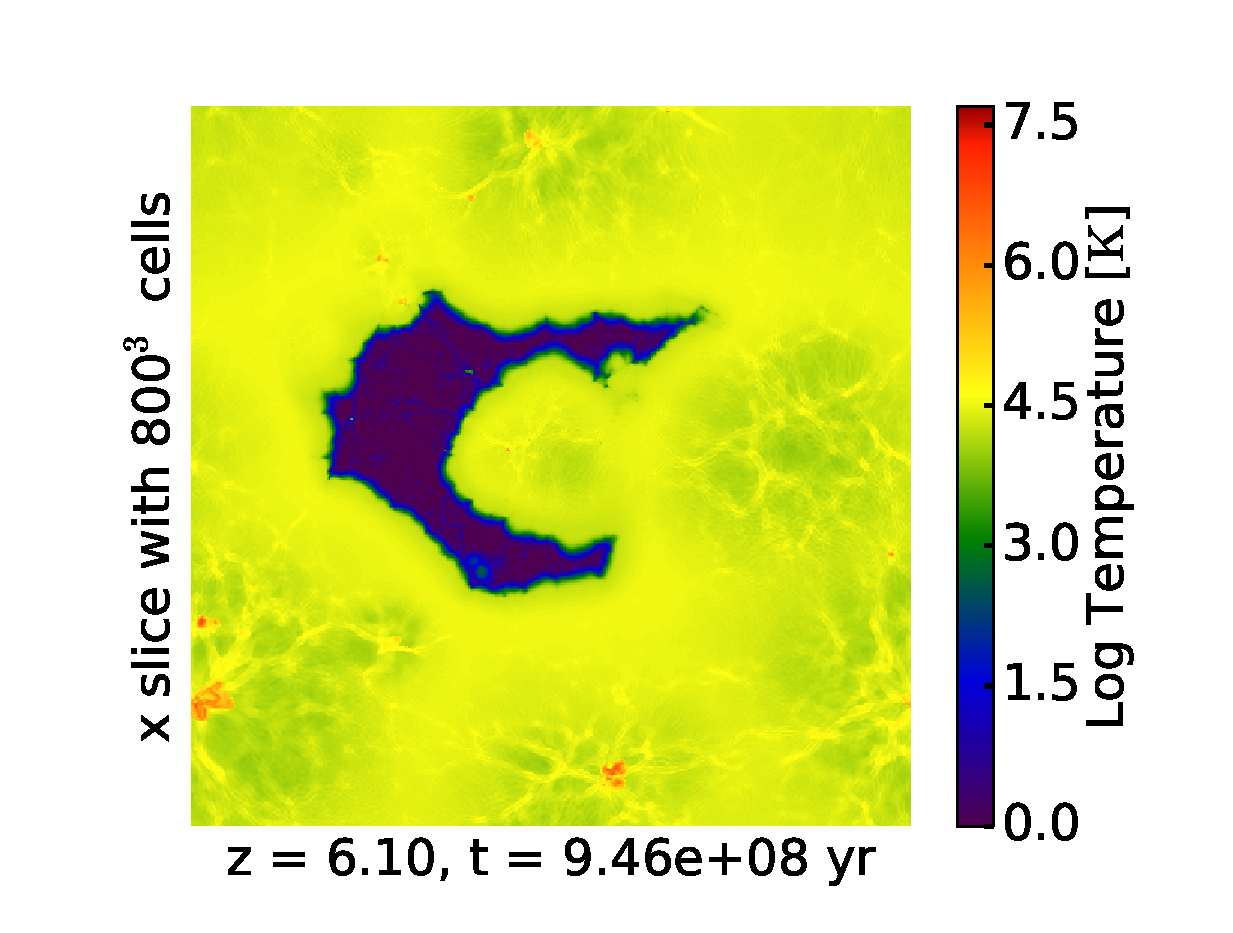
\includegraphics[trim = 10mm 0mm 7mm 7mm, clip, width=1.0\textwidth]{3_2_slice_Temperature_x_HD14475.eps}
	\end{minipage}
\hspace*{-2.00mm}
	\begin{minipage}[h]{0.33\linewidth}
	\centering
	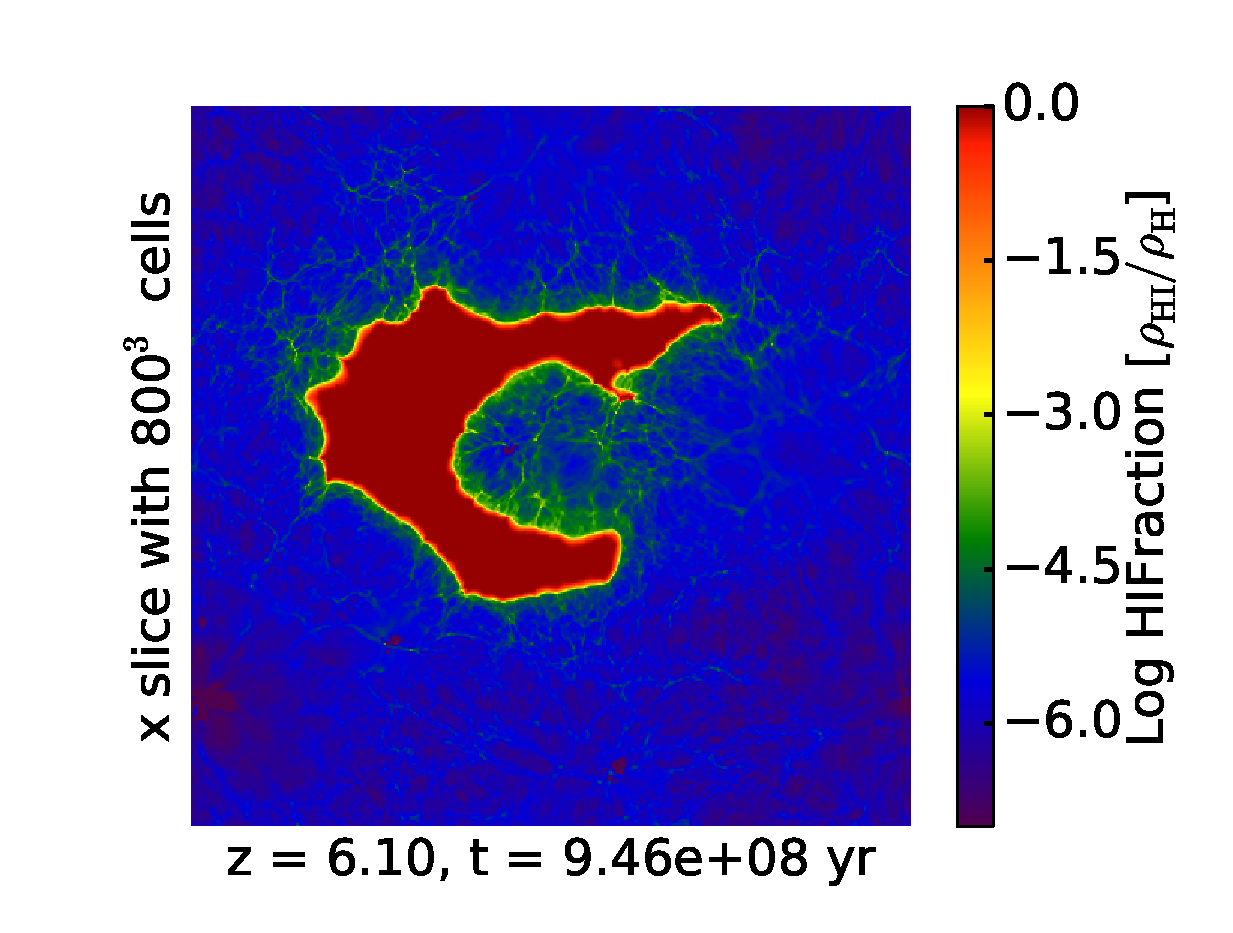
\includegraphics[trim = 10mm 0mm 7mm 7mm, clip, width=1.0\textwidth]{3_3_slice_HIFraction_x_HD14475.eps}
	\end{minipage}
\vspace*{-2.00mm}\\
	\begin{minipage}[h]{0.33\linewidth}
	\centering
	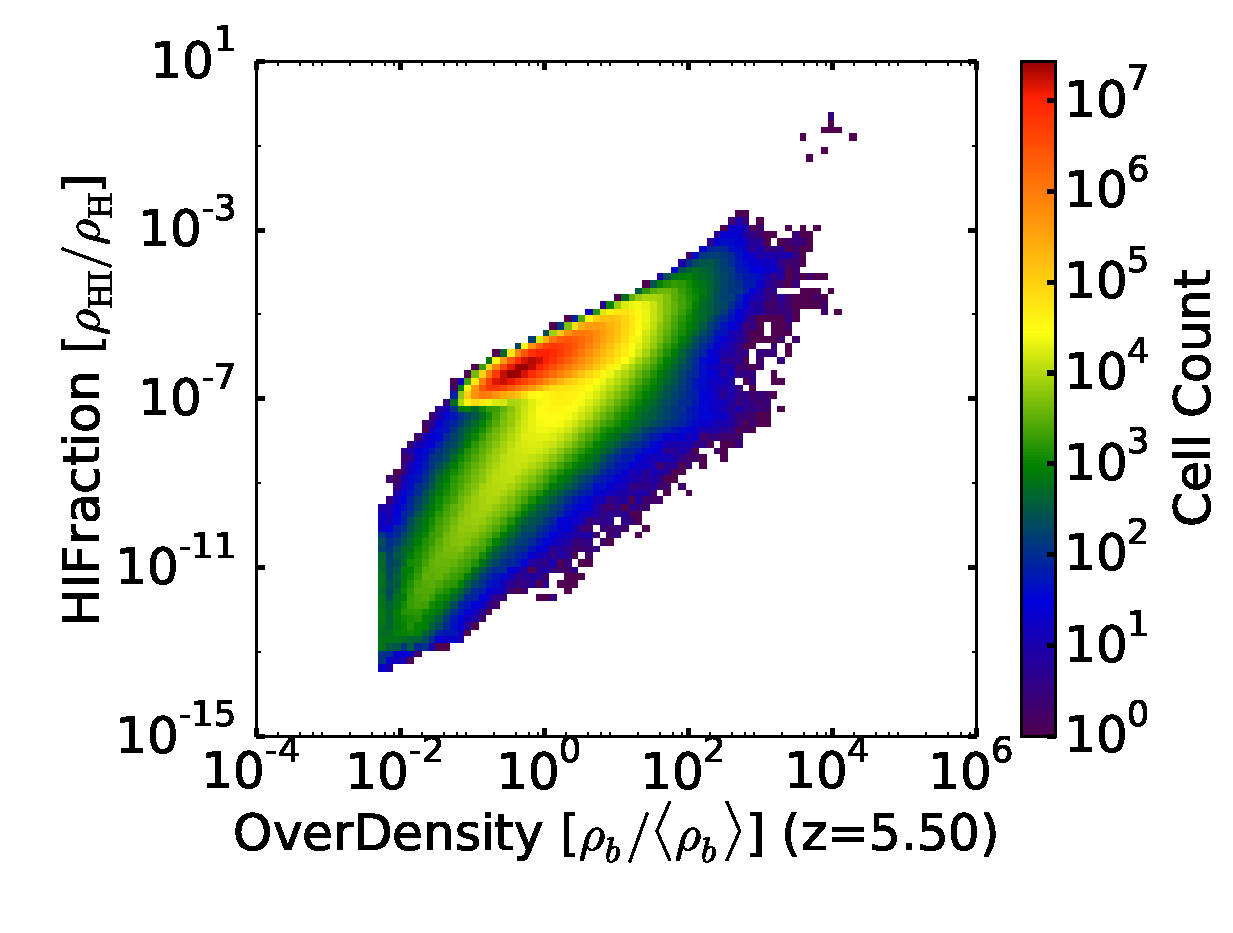
\includegraphics[trim = 7mm 9mm 1mm 7mm, clip, width=1.0\textwidth]{4_1_HD20125OverDensityHIFraction.eps}
	\end{minipage}
\hspace*{-2.00mm}
	\begin{minipage}[h]{0.33\linewidth}
	\centering
	\includegraphics[trim = 10mm 0mm 7mm 7mm, clip, width=1.0\textwidth]{4_2_slice_Temperature_x_HD20125.eps}
	\end{minipage}
\hspace*{-2.00mm}
	\begin{minipage}[h]{0.33\linewidth}
	\centering
	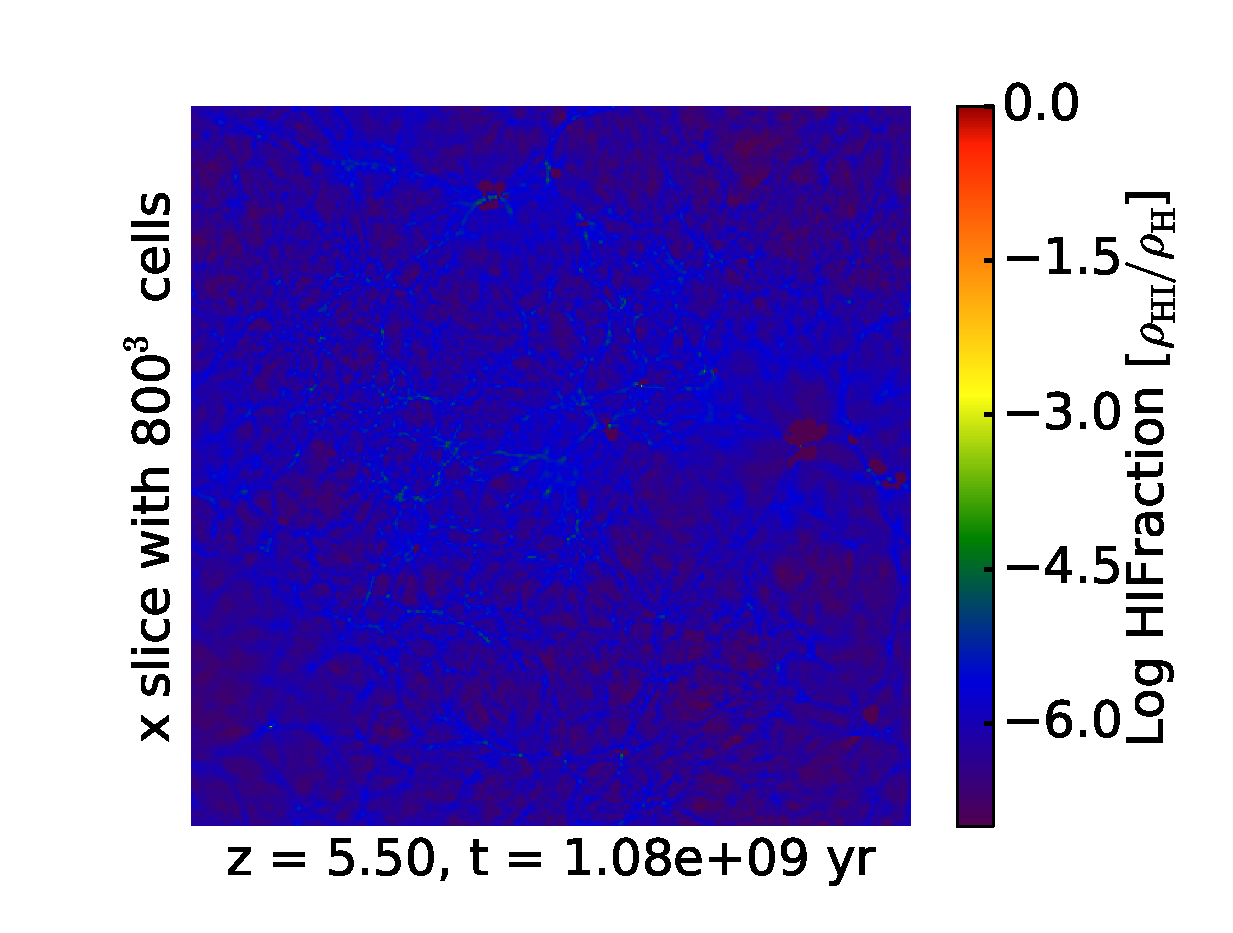
\includegraphics[trim = 10mm 0mm 7mm 7mm, clip, width=1.0\textwidth]{4_3_slice_HIFraction_x_HD20125.eps}
	\end{minipage}
\vspace*{-2.00mm}\\
	\begin{minipage}[h]{0.33\linewidth}
	\centering
	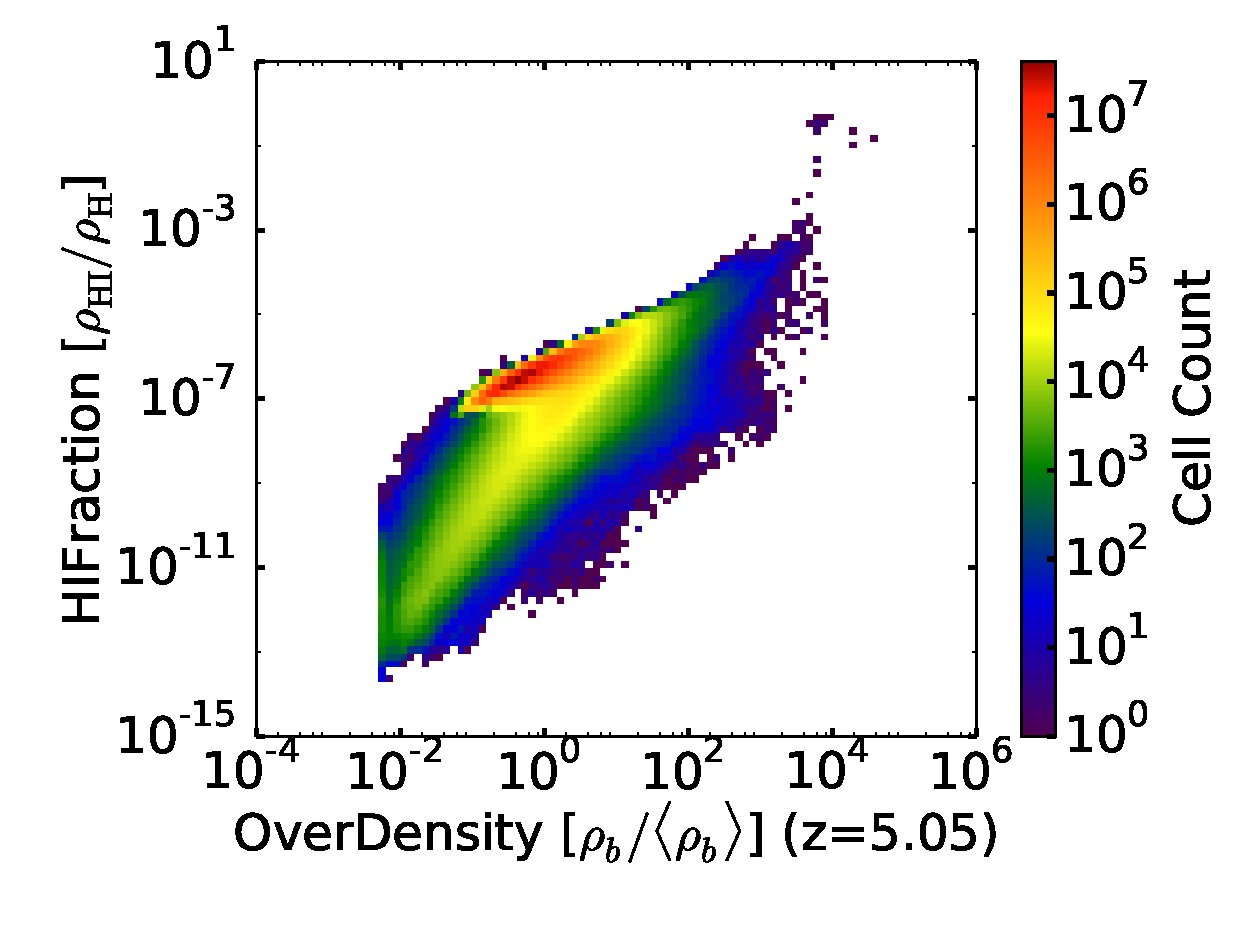
\includegraphics[trim = 7mm 9mm 1mm 7mm, clip, width=1.0\textwidth]{5_1_HD24175OverDensityHIFraction.eps}
	\end{minipage}
\hspace*{-2.00mm}
	\begin{minipage}[h]{0.33\linewidth}
	\centering
	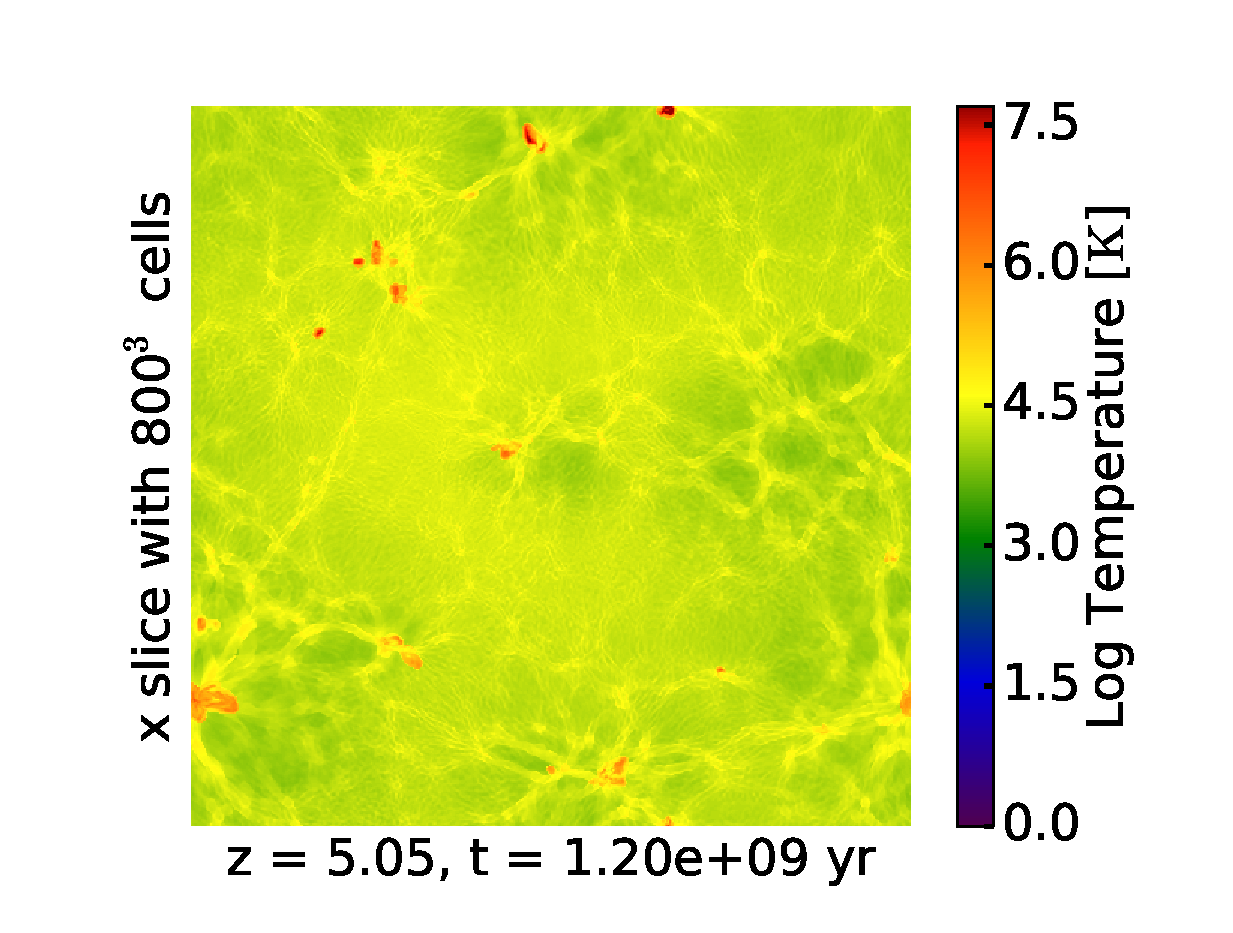
\includegraphics[trim = 10mm 0mm 7mm 7mm, clip, width=1.0\textwidth]{5_2_slice_Temperature_x_HD24175.eps}
	\end{minipage}
\hspace*{-2.00mm}
	\begin{minipage}[h]{0.33\linewidth}
	\centering
	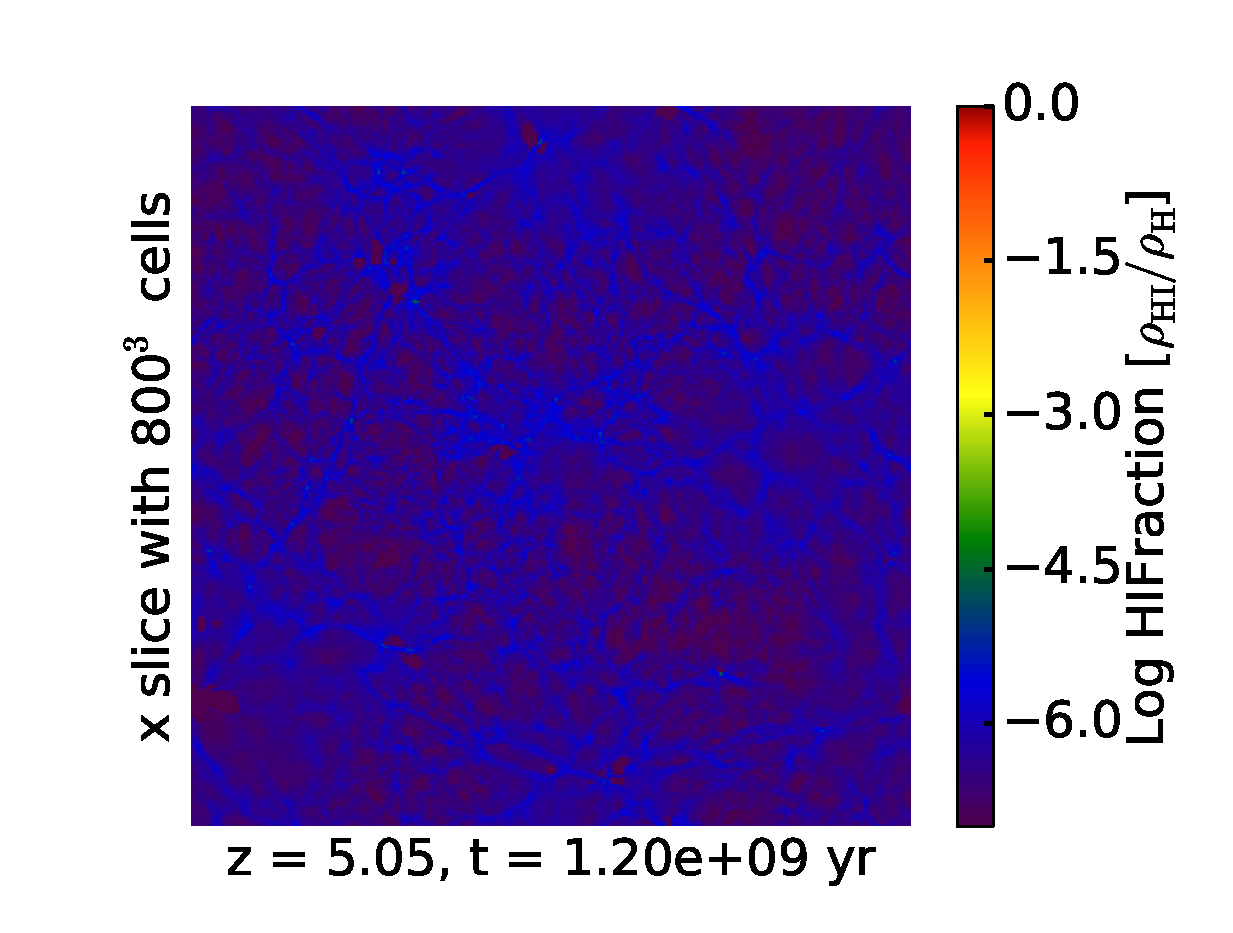
\includegraphics[trim = 10mm 0mm 7mm 7mm, clip, width=1.0\textwidth]{5_3_slice_HIFraction_x_HD24175.eps}
	\end{minipage}

	\caption{{\em Left}: Phase diagram of neutral hydrogen fraction versus baryon overdensity with decreasing redshift from top to bottom.  {\em Middle}: Slices of Log Temperature [K] through a region that remained mostly neutral until just before overlap at redshift of $\sim$5.8. {\em Right}: Slices of neutral hydrogen fraction through the same region as before.  Please refer to \S\ref{IOOI} for detailed description.}
  \label{NeutralPhase}
\end{figure*}


